\chapter{Modeling \& Results}

This chapter details the development and evaluation of statistical models for automated classification of email communications into spam and ham categories. The modeling approach employs Naive Bayes classification, a probabilistic technique particularly well-suited for text classification tasks due to its computational efficiency and effectiveness with high-dimensional sparse feature spaces.
Prior to model development, several preprocessing steps were implemented to structure the data appropriately: To facilitate unbiased model evaluation, the dataset was partitioned into training (80\%)  and testing (20\%) subsets.
The stratified sampling approach ensures that the class distribution is maintained in both training and testing subsets, preventing sampling bias that could distort evaluation metrics.
Next, we need to transforme unstructured text into numerical features using the Term Frequency-Inverse Document Frequency (TF-IDF) approach. This TF-IDF method captures both unigram and bigram features to model contextual patterns and limits feature space to 5,000 most informative features to prevent overfitting.

The Multinomial Naive Bayes classifier was selected as the primary modeling approach which match the prior distribution of the input tokenized text with its corresponding target class for posterior probability. 
K-Fold cross-validation was implemented to assess model stability across different data partitions.
Details of the cross-validation performance metrics are shown in Table \ref{tab:cv_metrics}.

\begin{table}[H]
\centering
\caption{Cross-validation performance metrics}
\label{tab:cv_metrics}
\begin{tabular}{lcc}
\toprule
\textbf{Metric} & \textbf{Value} & \textbf{Standard Deviation} \\
\midrule
Accuracy & 0.982 & 0.0112 \\
\bottomrule
\end{tabular}
\end{table}

The final model was evaluated on the held-out test set to assess generalization performance and tabulated in Table \ref{tab:test_metrics}.

\begin{table}[H]
\centering
\caption{Test set performance metrics}
\label{tab:test_metrics}
\begin{tabular}{lcccc}
\toprule
\textbf{Class} & \textbf{Precision} & \textbf{Recall} & \textbf{F1-Score} & \textbf{Support} \\
\midrule
Ham (0) & 0.99 & 0.99 & 0.99 & 1358 \\
Spam (1) & 0.97 & 0.96 & 0.97 & 484 \\
\midrule
Accuracy & \multicolumn{3}{c}{0.98} & 1842 \\
\bottomrule
\end{tabular}
\end{table}

The ROC curve is shown in Figure \ref{fig:roc_curve} with very high AUC score of 0.99.

\begin{figure}[H]
\centering
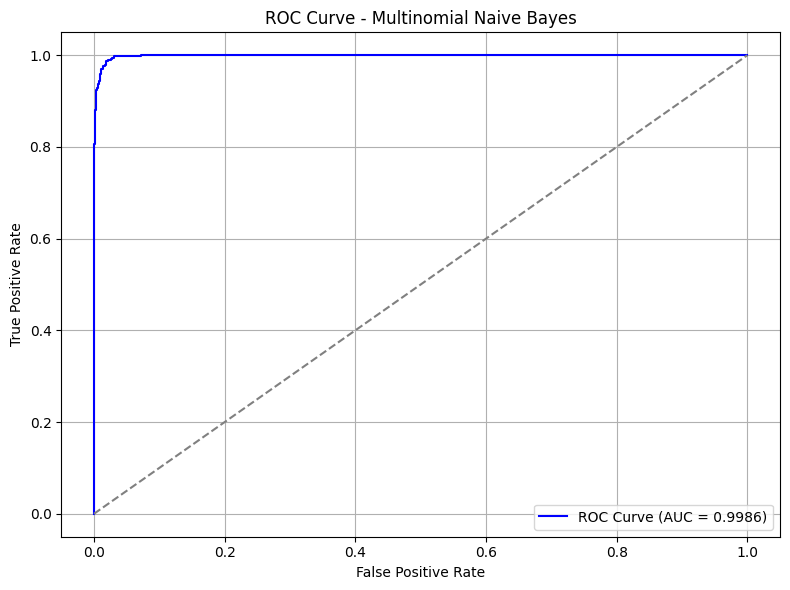
\includegraphics[width=0.7\textwidth]{figures/roc_curve.png}
\caption{ROC curve for test set predictions}
\label{fig:roc_curve}
\end{figure}

The Naive Bayes model facilitates interpretation of feature importance through examination of log-probability ratios. 
Top 20 most difference words between spam and ham domain are shown in Figure \ref{fig:spam_features} and Figure \ref{fig:ham_features}.

\begin{figure}[H]
\centering
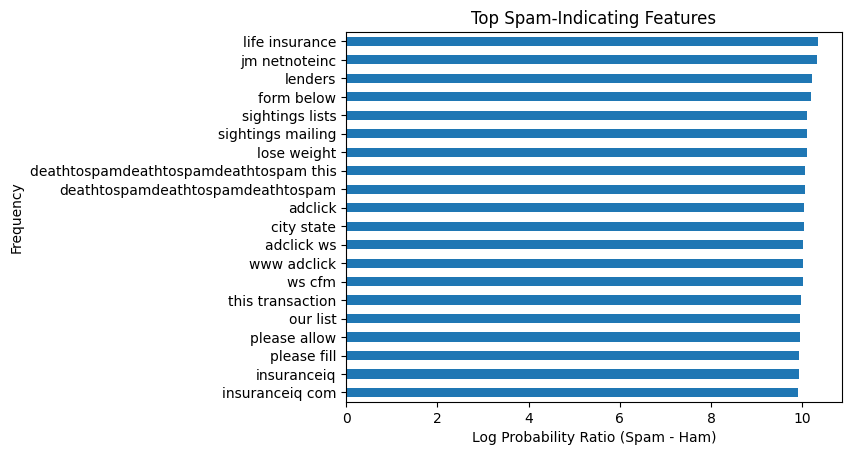
\includegraphics[width=1\textwidth]{figures/top_spam_words.png}
\caption{Top 20 most difference words between spam and ham domain}
\label{fig:spam_features}
\end{figure}

\begin{figure}[H]
    \centering
    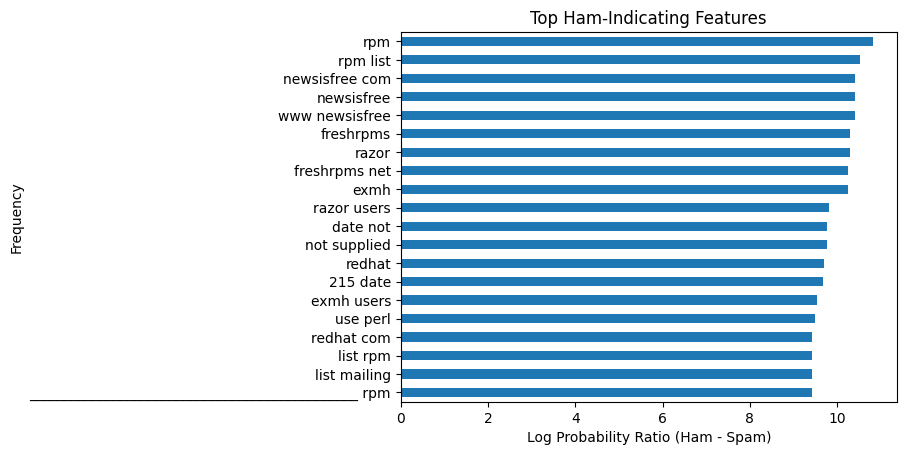
\includegraphics[width=1\textwidth]{figures/top_ham_words.png}
    \caption{Top 20 most difference words between ham and spam domain}
    \label{fig:ham_features}
    \end{figure}

This analysis reveals lexical features most strongly associated with spam classification, providing interpretability to the model's decision-making process.

Feature importance analysis revealed that marketing-related terms (free, click, offer) serve as primary discriminative features for classification. The error analysis identified specific challenges in handling short messages and technical content that could inform future model refinements. 